\section{Rule-based Heart Model Abstraction}
\label{ruleBasedHeartModelAbstraction}
Unlike system modeling in which there is only one concrete system, during environment modeling there are infinite number of environmental conditions that can be generalize by abstractions. In this section, we model the heart as the physiological environment for implantable pacemakers and try to cover different heart conditions and the closed-loop interactions between the heart and the pacemaker. Then using abstraction rules defined over physiological knowledge and principles for over-approximation we construct a series of heart model abstractions with different complexity and coverage. During the rule applications the merging of transition groups are documented thus can be used during model refinements.
\subsection{Electro-physiology (EP) Basics}
The heart generates periodic electrical impulses to control heart rates according to physiological needs. These impulses conduct through the heart, triggering coordinated muscle contractions and pump blood to the rest of the body. The underlying pattern and timing of these impulses determine the heart's rhythm and are the key to proper heart functions. Derangements in this rhythm are referred to as \emph{arrhythmia}, which impair the heart's ability to pump blood and compromise the patients' health. Arrhythmia are categorized into so-called \textsf{Tachycardia} and \textsf{Bradycardia}. Tachycardia features undesirable fast heart rate which results in inefficient blood pumping. Bradycardia features slow heart rate which results in insufficient blood supply. The electrical activities can be measured by inserting electrodes through the vein into the heart against the heart wall. Localized electrical activities can be measured, and the physicians can diagnose the heart conditions by delivering pacing sequence through the electrodes and observe the signal propagation. This procedure is referred to as Electrophysiological (EP) Testing  (\cite{josephson}) and the signals are referred to as electrograms (EGMs).

The implantable cardiac pacemakers are rhythm management devices designed to treat bradycardia. A typical dual chamber pacemaker has two leads inserted into the heart through the veins which can measure the local electrical activities of the right atrium and right ventricle, respectively. According to the timing between sensed impulses the pacemaker can deliver electrical pacing to the corresponding chamber to maintain proper heart rhythm.
\begin{figure}[!t]
\centering
		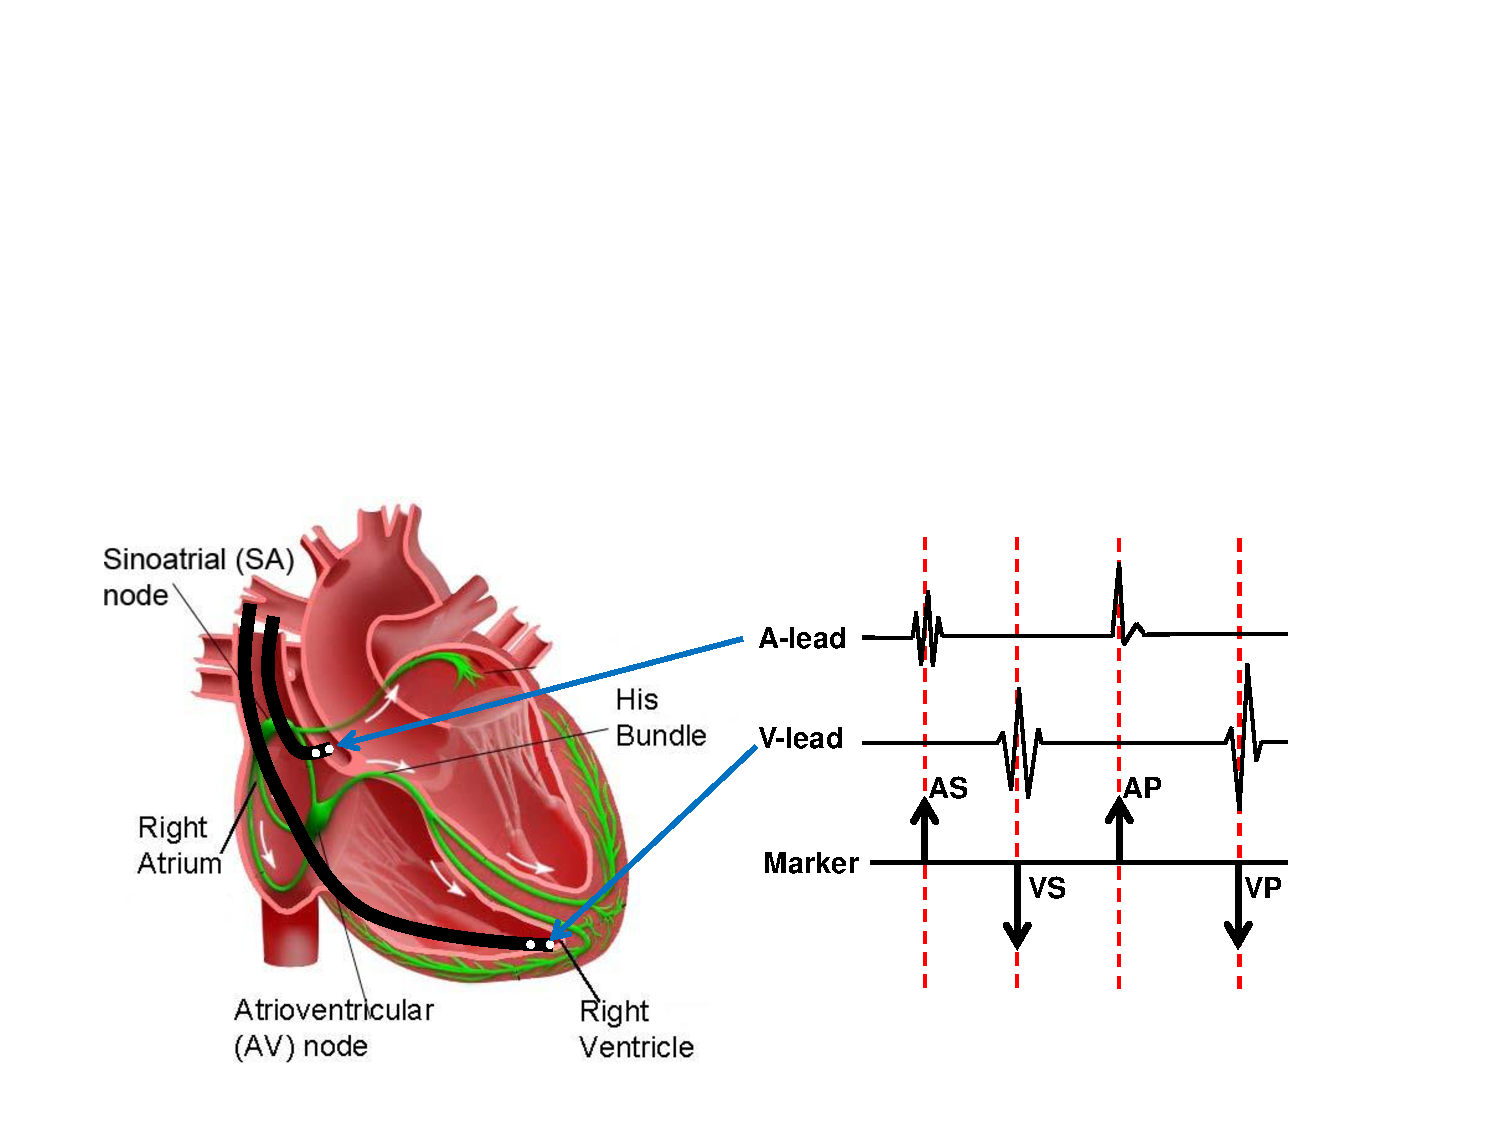
\includegraphics[width=0.7\textwidth]{figs/egm.pdf}
		
%\vspace{-10pt}
\caption{\small }
\label{fig:probes}
%\vspace{-15pt}
\end{figure} 

\subsection{Rule 1: Convert Reentry Circuits to Activation Nodes}
Within the conduction network of the heart, there can be multiple pathways between two locations, forming conduction loops. If the timing parameters of the tissue along the loop satisfy certain property, there can be scenarios in which an depolarization wave circling the circuit. The circuits are referred to as \emph{Reentry Circuits}. Since the time interval for an activation wave to circle a reentry circuit is usually less than the intrinsic heart cycle length, the heart rate will be "`hijacked"' by the reentry circuit once the cycling is triggered, causing tachycardia. Reentry is the most common mechanism for tachycardia which can be modeled by our heart models \cite{vhm_embc10}. 

The effect of reentry tachycardia is that activation signals coming out of the circuit with cycle length equals to the sum of conduction delays of the conduction paths forming the circuit. It is therefore reasonable to model a reentry circuit as a self-activation node with the self-activation range equal to the sum of conduction delays. For more complex structures with multiple circuits, the self-activation range will be the minimum of the shortest circuit to the maximum of the longest circuit. The detailed rule description and implementation can be found in \cite{regar_tech}.
\begin{figure}[!h]
		\centering
		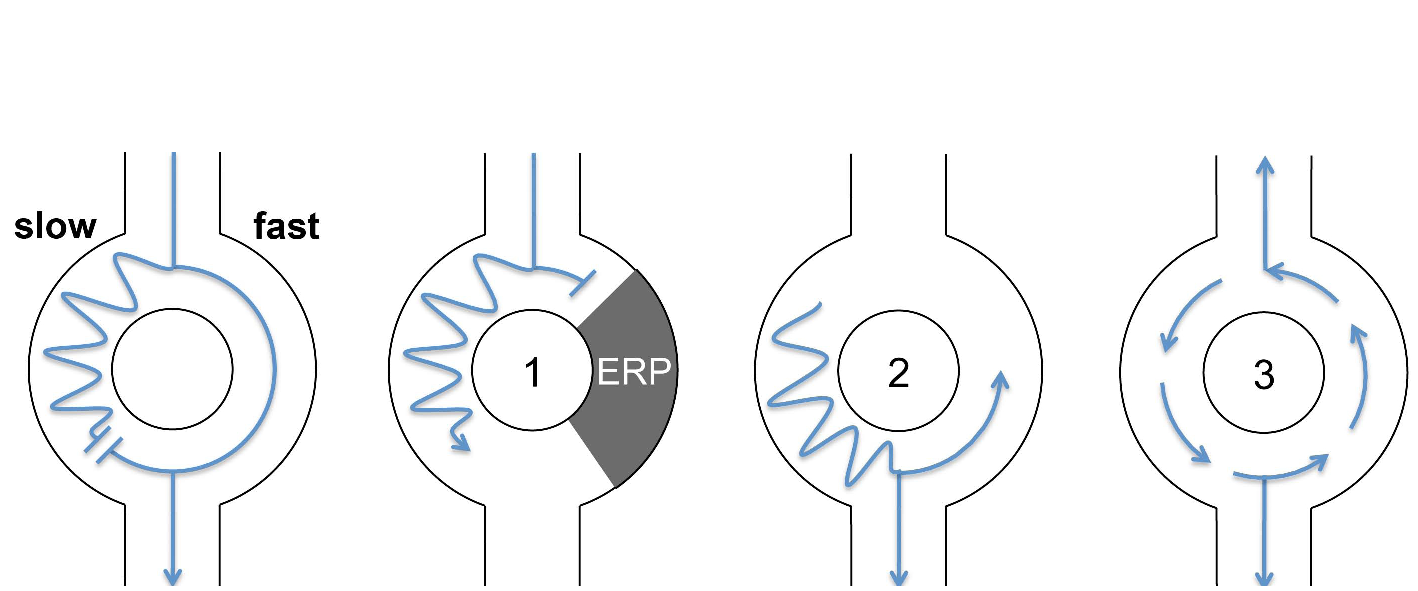
\includegraphics[width=0.6\textwidth]{figs/reentry.pdf}
		%\vspace{-5pt}
		\caption{\small Reentry Circuit}
		  %\vspace{-15pt}
		\label{fig:reentry}
\end{figure}

\subsection{Rule 2: Remove Irrelevant Structures}
The network of node and path automata can be viewed as a graph,with nodes as vertices, paths as edges with conduction delay as weight. After the loops within the topology are removed, the topology of the heart model is in form of tree. Within the network there are certain nodes that are more important in terms of model behaviors, we denote them as \emph{Nodes of Interests}, which include:
\begin{itemize}
	\item Nodes with self-activations
	\item Nodes which interact with the pacemaker
\end{itemize}
Graph algorithm can be performed on the heart model to identify the core structure. Shortest paths can be calculated among nodes of interests. All the nodes and paths along the shortest paths are regarded as core structure. All the other nodes and paths can be then removed without affecting the behaviors of the model. 

\subsection{Rule 3: Removing Unnecessary Non-self-activation Nodes}
The effect of non-self-activation nodes is blocking electrical events with interval shorter than its ERP period. If the self-activation nodes at both ends of a core path have self-activation interval longer than the maximum ERP period of nodes along the core path, the nodes can be removed.

For a core path from a self-activation node $N_1$ to another core node $N_2$, for any structure $P_1-N_n-P_2$ which $N_n$ is a non-self-activation node, if $N_n.ERP_{max}<min(N_1.Rest_{min},N_2.Rest_{min})$, replace $P_1-N_n-P_2$ with $P_3$ so that:
$$P_3.cond_{min}=P_1.cond_{min}+P_2.cond_{min}$$
$$P_3.cond_{max}=P_1.cond_{max}+P_2.cond_{max}$$
\subsection{Rule 4: Merge Parameter Ranges}
For heart models with the same node and path topology ($H_i,i=[1,p]$), they can be abstracted by a single heart model $H_a$ such that:
$$\forall i,j,H_a.\theta^j_{min}=min(H_i.\theta^j_{min})$$ 
$$\forall i,j,H_a.\theta^j_{max}=max(H_i.\theta^j_{max})$$ 
$H_a$ covers all possible behaviors, thus is an abstraction of $H_i, i\in [1,p]$. The added behaviors in the abstract model do not affect the number of transition groups
%\begin{algorithm}[tb]
%\caption{Rule 2: Removing Circuits}
%{\bf Input}: A heart model $H$ with nodes \\
%{\bf Output}: A heart model $H_a$ without circuits
%
%\begin{algorithmic}[1]
%
%\State Find all the loops in $H$ 
%\For {All the loops}
%\If {The loop contains core path(s)}
	%\If {The loop contains core node(s)}
		%\State 
	%\Else
	%\EndIf
		%\State
	%\Else
%\EndIf
 %
 %\State Compute $z_i^*=(x_i^*, t_i^*, \nu_i^*)$ 
 %\State $i=i+1$ 
%\EndFor\\
 %
%\end{algorithmic}
%\end{algorithm}
%if the circuit contains a core path
%
     %if the circuit contains a core node

\subsection{Rule 5: Merge Self-activation Nodes with Interaction Nodes}
The effect of self-activation nodes on the interaction of the pacemaker is triggering sensing events within certain delay. In this rule we merge all the self-activation nodes to their neariest interaction nodes. If there exists multiple self-activation nodes merging to the same interaction node, the parameters of the new model are determined following Rule 3.

\subsection{Rule 6: Replace Blocking With Non-deterministic Conduction}
The effect of a node automaton blocking an activation signal is equivalent to a path not conducting. So we designed new abstract node and path automata $N1$ and $P1$. For any $P_1-N_n-P_2$, it can be replaced by a $P$ with:
$$P.cond_{min}=P_1.cond_{min}+P_2.cond_{min}$$
$$P.cond_{max}=P_1.cond_{max}+P_2.cond_{max}$$
For any self-activation node $N$:
$$N'.rest_{min}=N.ERP_{min}+N.rest_{min}$$
$$N'.rest_{max}=N.ERP_{max}+N.rest_{max}$$

\begin{figure}[!h]
		\centering
		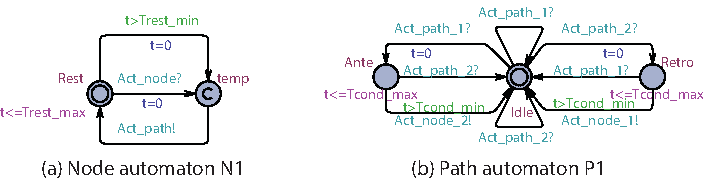
\includegraphics[width=0.9\textwidth]{figs/rule5.pdf}
		%\vspace{-5pt}
		\caption{\small Heart Model Abstractions}
		  %\vspace{-15pt}
		\label{fig:rule5}
\end{figure}

\subsection{Rule 7: Replace Conductions With Self-activation}
The effect of conduction path is to connect activations from a self-activation node to another. By setting the interval between self-activations to $[0,\infty]$ the observable behaviors of the heart will not change.

For all node $N$, $N.Rest_{min}=0,N.Rest_{max}=\infty$ and delete all paths.
\begin{figure}[!h]
		\centering
		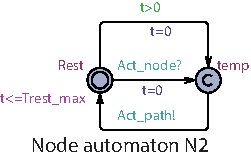
\includegraphics[width=0.3\textwidth]{figs/rule6.pdf}
		%\vspace{-5pt}
		\caption{\small Heart Model Abstractions}
		  %\vspace{-15pt}
		\label{fig:rule6}
\end{figure}

\subsection{Rule Application Example}
In this section we demonstrate 

$$NA\_self=\{SA\_self,AVNRT\_self,AF\_self,PAC\_self\}$$
$$NV\_self=\{PVC\_self,VF\_self,VT\_self\}$$
$$NA-AV'\_cond=\{SA-AV\_cond\}$$
$$AV'-NV\_cond=\{AV-RBB\_cond,RBB-RVA\_cond\}$$
Apply Rule 6:
$$NA'\_self=\{NA\_self\}$$
$$NV'\_self=\{NV\_self\}$$
$$NA'-NV'\_cond=\{AV'\_block,NA-AV'\_cond,AV'-NV\_cond\}$$
Apply Rule 7:
$$NA''\_self=\{NA'\_self,NA'-NV'\_cond\}$$
$$NV''\_self=\{NV'\_self,NA'-NV'\_cond\}$$
\begin{figure}[!t]
		\centering
		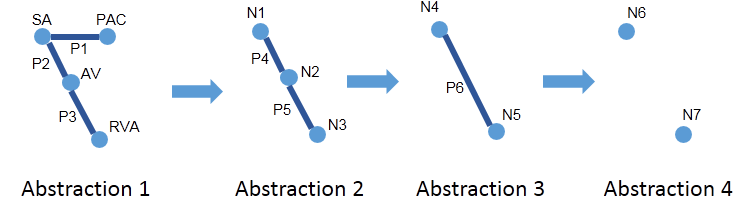
\includegraphics[width=0.9\textwidth]{figs/abs.png}
		%\vspace{-5pt}
		\caption{\small Heart Model Abstractions}
		  %\vspace{-15pt}
		\label{fig:abs_exam}
\end{figure}







